\chapter{Automatic Synthesizer Programming}
\label{chapter:asp-background}

In the previous chapter, some of the specific challenges in synthesizer programming were identified along with the desire among synthesizer users for improved user interfaces and supportive tools. The field of automatic synthesizer programming emerged from the desire to solve these challenges and to find more intuitive answers for the question "How do I create \rule{1cm}{0.15mm} sound using \rule{1cm}{0.15mm} synthesizer?" James Justice \cite{justice1979analytic} was one of the first to try to answer this question in the late 1970s. Justice's work used analytic methods to estimate the parameters for the FM algorithm \cite{chowning1973synthesis}. This is an example of inverse synthesis, or sound matching \cite{horner1993machine}, where a system estimates synthesizer parameters to replicate a target sound as closely as possible. Since then a large volume of work in automatic synthesizer programming has been published, exploring a variety of synthesis techniques, algorithmic methods, and user interaction approaches. This chapter provides an overview of the field and surveys some of the more popular methods that have been explored over the more than 40 years that automatic synthesizer programming has been an active area of research.

To the author's knowledge, at the time of writing there are no published works that provide an overview of the field of automatic synthesizer programming. The term \textit{automatic synthesizer programming} was first coined by Matthew Yee-King in work on sound matching using a genetic algorithm \cite{yee2008synthbot}. This term has typically been used to refer to approaches that are focused on algorithmic techniques for sound matching or inverse synthesis problems. For the purpose of this thesis, automatic synthesizer programming (ASP) refers to any system that uses technology to support the process of programming an audio synthesizer. This includes all of the approaches to inverse synthesis, as well as other interaction paradigms, which will be reviewed here.

\section{Problem Formulation}
The synthesizer programming problem is fundamentally a human computer interaction (HCI) problem. Currently, in order to use a synthesizer, users are expected to learn the domain language of the synthesizer they are using, as opposed to communicating ideas to their synthesizer in a way that suits their own creative needs. Creativity support is an emerging field of study that is interested in addressing HCI issues similar to this in creative domains. It is focused on the development of tools that enable and enhance the creative output of an individual or group -- both novices and experts. Creativity support tools (CSTs) \cite{shneiderman2007creativity} span a wide array of application domains including visual art, textiles, cooking, and music. A central question that CSTs ask is: "How can designers of programming interfaces, interactive tools, and rich social environments enable more people to be more creative more often?" \cite{shneiderman2007creativity}. Reframing this question in the context of automatic synthesizer programming research results in the following question:
\begin{quote}
    How can designers of \textit{synthesizer} programming interfaces enable more people to be more creative more often?
    %\footnote{Rich social environments has been left out of this question as it doesn't relate directly to the techniques reviewed here, however that doesn't not exclude social environments from contributing to the experience of programming synthesizers. [so and so provides information on that - find reference]}
\end{quote}

Answers to this question are related to the conceptual distance that was identified as one of the central challenges of synthesizer programming in the previous chapter. The distance between the perceptual/semantic space and the parameter space of a synthesizer is large and complex, requiring users to obtain large amounts of domain knowledge to effectively learn how to translate between those spaces themselves. Previous work in automatic synthesizer programming has sought to address this conceptual gap from a variety of different angles. This chapter reviews the main approaches to this problem.

\section{Approaches}
% Does this fit it \cite{paz2020fly}?

\label{sec:asp-approaches}
A typical automatic synthesizer programming system is an additional layer of abstraction on top of the control interface of an existing synthesizer. The goal of this abstraction is to help bridge the conceptual distance between the parameter space and the perceptual and semantic space. Similar to how synthesizer control interfaces create a mapping from the parameter space to the synthesis engine, interfaces of automatic synthesizer programming systems present an abstracted higher-level model of the parameter space to a user and create a mapping to the parameter space. Figure \ref{fig:asp_bridge_the_gap} shows an updated diagram of the synthesizer user interaction model from the previous chapter (see figure \ref{fig:synth_conceptual_dist}) with an automatic synthesizer programming system inserted that assists in the translation from the perceptual/semantic space to the parameter space of a synthesizer.


\begin{figure}
    \centering
    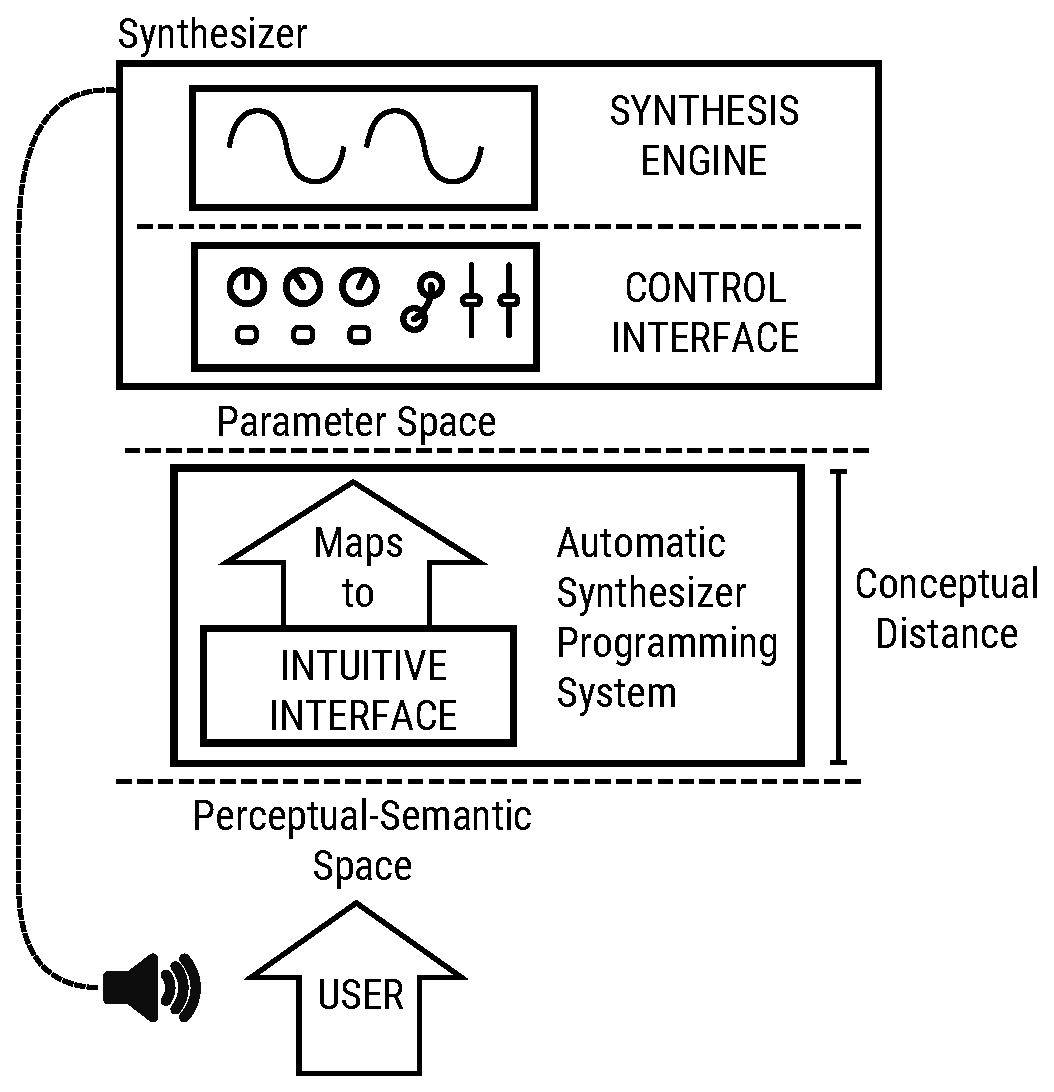
\includegraphics[width=0.6\textwidth]{figures/background/asp_bridging_the_gap.eps}
    \caption{Automatic synthesizer programming systems assist in translating between the parameter space and perceptual-semantic space of a synthesizer. This diagram updates figure \ref{fig:synth_conceptual_dist} from the previous chapter and shows how an automatic synthesizer programming system fits with an existing synthesizer and provides an intuitive interface that maps to the parameter space.}
    \label{fig:asp_bridge_the_gap}
\end{figure}

A number of different interface approaches have been explored in previous ASP research. Pardo \textit{et al.} \cite{pardo2019learning} presented a framework for classifying different interaction paradigms within audio production tools. The development of this framework was based on how musicians and audio engineers communicate auditory concepts and included four different types of interaction styles: 1) evaluation, 2) descriptive words, 3) vocal imitations, and 4) exploration. Pardo \textit{et al.} evaluated four different examples of audio production software with \textit{natural} interfaces that attempted to bridge the gap between the parameter space and perceptual/semantic space. Each system was categorized under one or more of the interaction paradigms. These categorizations are useful for understanding the different approaches to ASP interfaces that have been proposed in previous work. For ASP systems, two additional categories are included: \textit{example-based} interfaces and \textit{intuitive controls}. There are six interaction paradigms for automatic synthesizer programming:

\begin{enumerate}
    \item example-based interfaces (users provide an audio example of the sound that they want to play);
    \item evaluation interfaces (users compare and evaluate results of different parameter settings to help guide the selection process);
    \item using descriptive words (semantic description of the desired result);
    \item vocal imitations (users imitate the sound that they desire);
    \item intuitive controls (higher-level parameters, or macro parameters, are provided that have a complex mapping to to the lower level parameters); and
    \item exploration interfaces (a number of different results are produced and provided to the user in a way for them to explore).
\end{enumerate}

An overview of each of the approaches and related work is provided in the following sections. While previous work is introduced as a being a particular interaction style, there is overlap between each of these styles and many applications utilize more than one approach. For example, an evaluation-based interface that presents a user with a set of options for ranking could also be classified as an exploration-based interface because it supports the user in listening to a variety of different solutions. As a result, some work may be introduced as utilizing a specific style, and then repeated in another. Example-based approaches represent the largest portion of related work in automatic synthesizer programming and provide technical context for the other approaches discussed in this thesis.

\section{Example-Based Interfaces}
\label{sec:asp-example-based}
The example-based paradigm for automatic synthesizer programming has dominated the landscape of previous work. Approaches that fall into this category are typically referred to as \textbf{sound matching} or \textbf{inverse synthesis}. The goal of these systems are to find a parameter setting for a synthesizer that sounds as close as possible to a given example target sound. 

The first research in this vein was conducted out of a desire to develop a deeper understanding of the complex relationship between the perceptual / semantic space and the parameter space of a synthesizer, and to learn more intuitive methods for synthesizer programming. In the late 70s through to the early 90s, several researchers studied analytic methods to attempt to reverse engineer parameter settings for FM synthesis \cite{justice1979analytic, beauchamp1982synthesis, payne1987microcomputer} and non-linear synthesis \cite{delprat1990parameter}. In 1993, Andrew Horner conducted one of the first synthesizer sound matching experiments for FM synthesis using an artificial intelligence approach \cite{horner1993machine}. Horner used a genetic algorithm (GA) to search through the parameter space and to find the optimal parameter settings to match target instrumental sounds, including trumpets and guitars.

A typical inverse synthesis system involves the following steps: 1) the system receives a raw audio target, 2) the audio is processed and transformed into a representation for input to an algorithm, and 3) an algorithm receives the input representation and outputs parameter settings to match the audio target.

% TODO
%[Create a diagram of this process]

\subsection{Audio Representations}
% This is kind of crap. Need to figure out how to introduce this -- perhaps this is a background section.
Generally, the first step in a typical inverse synthesis system is to convert the raw input audio into a representation that exposes relevant features for the proceeding algorithm. What defines a relevant feature in the context of audio analysis for synthesizer programming is an open question to which a wide variety of approaches have been explored. Most commonly, audio is transformed from a time-domain representation to a temporal-spectral representation that exposes the time-varying frequency components of the target sound. Previous work has used the temporal-spectral representation produced by the short-time Fourier transform \cite{horner1995wavetable, horner1995envelope, horner1996piecewise, chinen2007genesynth, yee2007evolving, barkan2019inversynth}. 

Audio features extracted from temporal, spectral, and temporal-spectral representations are reviewed by Peeters \cite{peeters2004large} and have been used in inverse synthesizer research \cite{mintz2007toward, stowell2010making, mcartwright2014, blancas2014sound}. Mel-frequency cepstral coefficients (MFCCs) -- initially used for speech processing research -- provide a compact representation of the shape of a spectrum, and have been used in work by Yee-King \cite{yee2008synthbot}, Heise \cite{ heise2009automatic}, Roth \cite{roth2011comparison}, and Smith \cite{smith2017play}. Transforms that attempt to model perceptual attributes of human-hearing have also been explored, including log-scaled Mel-spectrograms \cite{zhang2018visualization}, which feature loudness and frequency scales that are more reflective of the human auditory system.

A more recent approach to extracting audio representations is to learn them using deep learning networks, a process called representation learning  \cite{bengio2013representation}. Barkan \textit{et al.} explored using a convolutional neural network to learn features directly from time-domain audio \cite{barkan2019inversynth}. Beyond the context of synthesizers, several researchers have built and trained models for generating audio representations \cite{cramer:learnmore:icassp:19, drossos:icml:2020, engel2017neural}, which provide promising options for future automatic synthesize programming approaches -- both as off-the-shelf solutions or for inspiration for learning custom representations specifically for synthesizer sounds.

\subsection{Approaches to Inverse Synthesis}
Algorithmic approaches that have been used for parameter estimation in inverse synthesis can be loosely categorized into search and modelling methods. Search algorithms, which include genetic algorithms, estimate an optimal parameter settings by performing a structured search of the parameter space. Modelling methods, on the other hand, which have become more popular in recent years with the growth of deep learning, attempt to model the parameter space in order to estimate parameter settings. Other methods beyond search and modelling approaches that have been used in ASP research include fuzzy logic \cite{mitchell2005frequency, hamadicharef2012intelligent}, linear coding \cite{mintz2007toward}, and query approaches \cite{mcartwright2014}.

\subsection{Search Based Methods}
The most popular search methods used in automatic synthesizer programming research are genetic algorithms. A genetic algorithm (GA) is a method for solving an optimization problem using techniques based on the principles of Darwinian evolution, and is part of a broader class of evolutionary algorithms \cite{whitley1994genetic}. In a GA, a potential solution (an individual) is represented by its \textit{genotype} and \textit{phenotype}. In biology the genotype of an organism refers to its genetic makeup or set of genes, and the phenotype refers to the observable properties of that organism. In the context of synthesizer programming, the genotype is the set of parameters, represented by an array of numeric values, and the phenotype is the auditory result. 

During optimization with a GA, an initial set of individuals is randomly generated, and then iteratively evolved by subjecting the genotypes to a set of biologically inspired processes including selection, breeding (cross-over), and mutation. Individuals are ranked using an evaluation function that measures the $fitness$ of a given solution, which is calculated on the phenotype. The objective of a GA is to minimize that value (or maximize it, depending on the problem definition). The best candidates are selected for further evolution until either an optimal solution is found or a set number of iterations has been completed.

In the case of sound matching, the \textit{fitness} of a potential solution is determined by measuring the error with regards to the phenotype of that solution and a target. The phenotype is usually represented using a time-frequency representation of the resulting audio; previous solutions have used spectrograms from the STFT \cite{horner1993machine, tatar2016automatic, masudo2021quality} as well as mel-frequency cepstral coefficients (MFCCs) \cite{yee2008synthbot, roth2011comparison, macret2014automatic, smith2017play}.

% Can we add some of the single objective GAs here?
Tatar \textit{et al.} introduced the use of a multi-objective GA (MOGA) for synthesizer sound matching that used three different methods for representing phenotypes: the STFT, Fast Fourier Transform (FFT), and signal envelope \cite{tatar2016automatic}. Each phenotype representation was used in a different fitness function for an objective; therefore, the MOGA used by Tatat \textit{et al.} had three objectives. In their work, they sought to automatically program a popular, portable synthesizer called the OP-1\footnote{\url{https://teenage.engineering/products/op-1}} developed by Teenage Engineering.

The goal of a MOGA is to find a set of \textit{pareto-optimal} solutions. A solution is \textit{pareto-optimal} when no other solution is better than it for all the fitness values and the set of \textit{pareto-optimal} solutions is called the \textit{pareto-front}. There are multiple different approaches to solving the optimization problem presented by a MOGA, popular solutions include the NSGA II \cite{deb2002fast} and NSGA III \cite{deb2013evolutionary} algorithms. Tatar \textit{et al.}'s approach used an NSGA III. 

A more recent solution proposed by Masuda and Saito \cite{masudo2021quality} utilized the NSGA II algorithm. The MOGA in their work had two objectives: the first was to minimize the error between the power spectrograms of the phenotypes, and the second was to maximize the diversity of phenotpyes as measured by a \textit{behaviour characteristic}, which was represented by the spectral centroid and spectral flatness. From this dual-objective arises the concept of \textit{quality diversity}: the \textit{pareto-front} should contain solutions that are not only of high-quality (close to the target), but also should represent a diverse selection of solutions. In the context of automatic synthesizer programming, presenting a user with a set of potential solutions based on quality diversity could be beneficial in the sense that it would allow them to evaluate potential candidates from a wider range of possibilities that are close to their target.

% [I like the image in Masuda and Saito 's paper -- perhaps can grab that]

In addition to GAs, other search-based techniques that have been used for sound matching include Particle Swarm Optimization (PSO) \cite{heise2009automatic} and Hill-Climbing \cite{roth2011comparison, luke2019stochastic}.

\subsection{Deep Learning Methods}
Deep learning is subset of machine learning that utilizes artificial neural networks to learn patterns in data and make predictions based on those patterns \cite{lecun2015deep}. Deep learning models contain multiple layers comprised of simple non-linear modules. Through iterative training, the layers are able to extract features from raw input data and learn intricate patterns in high-dimensional data. These multi-layer models have enabled deep learning models to excel at complex tasks including image recognition, speech recognition, and music related tasks such as audio source separation \cite{spleeter2019} and pitch detection \cite{kim2018crepe}.

In the context of an automatic synthesizer programming inverse synthesis experiment, a deep learning model accepts an audio signal as input and predicts synthesizer parameter settings to replicate that audio signal. Audio signals are often pre-processed using audio feature extraction or transformed into a time-frequency representation, although some approaches use raw time-domain audio \cite{barkan2019inversynth}. Models are trained using a large set of example sounds generated from a synthesizer and use the parameter settings that generated a particular sound as the ground truth. During training, the loss is used to evaluate how well a model is learning and to optimize the parameters of the model through gradient descent. The loss is calculated using a loss function, which is computed using the error between predicted parameter settings and the actual parameter settings (the ground truth). In deep learning, models are grouped into discriminative models, which learn decision boundaries through observed data, or generative models, which learn the distribution of observed data. Related automatic synthesize programming approaches to the inverse synthesis problem have explored both types of models, and will be reviewed in the following sections.

\subsubsection{Discriminative Models}
One of the first works on the application of deep learning to the inverse synthesis problem was published by Matthew Yee-King et al. \cite{yee2018automatic} in 2018. The main contribution of their work was an experiment that showed the effectiveness of a type of recurrent neural networks (RNN) called long short-term memory (LSTM) networks at sound matching on an FM synthesizer audio plugin. RNNs were developed to handle time-series data and to receive ordered data which is successively fed into the network architecture. As data is fed into the networks, activation states are stored internally and help to provide temporal context in latter stages of computation. RNNs have been particularly successful for audio generation problems \cite{oord2016wavenet, engel2017neural}. 

Yee-King \textit{et al.} also experimented with additional machine learning techniques including genetic algorithm (GA), Hill-climber, and  multi-layer perceptron (MLP) methods. They also compared two RNN models: a regular LSTM network as well as a modified LSTM network that had a bi-directional LSTM layer and as several highway layers. They called this network an LSTM++. Their methodology compared a set of algorithms on a series of successively more challenging problems on the open-source FM synthesizer Dexed\footnote{\url{https://asb2m10.github.io/dexed/}}. Each problem was focused on programming a subset of the parameters in Dexed; a larger subset was used for each successive problem. A dataset of audio samples paired with the parameters used to generate the audio was created for training each of the deep learning models. Mel-frequency Cepstral Coefficients (MFCCs) were used as input for each of the models. The results were evaluated by looking at the error between MFCCs from target sound and a predicted sound. Results showed that the hill-climber algorithm and the LSTM++ model performed the best. The LSTM++ model showed significant improvements over the other deep learning methods; however, the hill-climber performed the best on a majority of the tasks.

Barkan et al. explored convolutional neural networks (CNNs) applied to the inverse synthesis problem in their work which presented InverSynth \cite{barkan2019deep}. The CNN has been used extensively for image related deep learning tasks and has recently been used successfully in music and audio related tasks, including music genre classification \cite{choi2016automatic} and neural audio generation \cite{donahue2018adversarial}. A key feature of CNNs is the use of shared filters that perform convolutions and produce representations at various levels of specificity. The shared filters allowed them to process large input data such as images and audio with relatively few parameters compared to their fully connected counterparts. 

In their work, Barkan et al. experiment with several different CNN architectures and compare them to a few different fully-connected networks. The focus of their research was performing inverse synthesis on a custom four oscillator FM synthesizer. They framed the inverse synthesis problem as a classification problem and quantized each of the 23 continuous synthesizer parameters into 16 discrete states. As input, they experimented with spectrograms from the STFT as well as raw time-domain audio. Because of the size of these inputs, they created different input representations for the fully-connected networks using a selection of hand-picked audio features defined in work by Itoyama et al. \cite{itoyama2014parameter}.

Micheeltree and Koike introduced an interesting approach to programming Serum\footnote{\url{https://xferrecords.com/products/serum}}, a popular VST wavetable synthesizer \cite{mitcheltree2021serumrnn}. They focused on the audio effects processing chain that follows the initial synthesis stage and explored using an ensemble of CNN models that worked together to select and adjust the effects. Each model in the ensemble was responsible for a single effects module (compressor, distortion, equalizer, phaser, or a reverb) and another model was responsible for selecting the ordering of each of the individual effects modules. Micheltree and Koike hypothesized that this approach was similar to how a human might select and program a synthesizer audio effect chain. Their approach also provided insight into the intermediate steps of programming a synthesizer that could be useful for educational purposes.

\subsubsection{Generative Models}
% Expand on the Esling approach?
Esling et al. recently presented a novel application called $FlowSynth$ that uses a generative model based on Variational Auto-Encoders (VAE) and Normalizing Flows \cite{esling2020flow}. Building on FlowSynth, Le Vaillant \textit{et al.} also used a generative approach and explored programming a software implementation of the Yamaha DX7 using a VAE with normalizing flows \cite{le2021improving}. Their work includes two important insights to the process of training a syntesizer programming model. The first involves the dataset that was used: they identified that previous research generated datasets of synthesizer + preset pairs by randomly sampling the parameter space and introduced a dataset of presets designed by humans. The second important insight related to how input is provided to the model. Their model received a multi-channel input that consisted of six different outputs from the same preset, played using different MIDI inputs. This factor is important because it identifies and takes into consideration that a synthesizer can have the exact same parameter setting, but varying the MIDI pitch and velocity that is used to trigger the sound will result in a different sound. Using this multi-channel input allowed the network to learn how a single synthesizer preset may respond to different MIDI input.

\section{Evaluation Interfaces}
Evaluation interfaces for synthesizer programming allow a user to compare the results from multiple parameter settings to help them navigate and select a desired setting. One approach to evaluation style interfaces is through the use of interace genetic agorithms (IGAs) \cite{johnson1999exploring, dahlstedt2001creating, yee2016use}. In contrast to the GAs introduced in the example-based systems, the evaluation function in an IGA relies on user feedback during each iteration as opposed to measuring error between a candidate and a target. This allows a user to provide feedback to the system and participate in the process of finding a sound. IGAs also facilitate exploration as they can produce a large variety of novel examples in a short period of time and help a user explore different aspects of the parameter space. Figure \ref{fig:evosynth} shows an example an evaluation-based interface called EvoSynth developed by Matthew Yee-King \cite{yee2016use}. EvoSynth initially presents a user with a number of randomly selected examples, which they can listen to and iterate upon by selecting multiple examples to "breed" together. EvoSynth is web-based and at the time of writing is still available online\footnote{\url{http://www.yeeking.net/evosynth/}}.

\begin{figure}[ht]
    \centering
    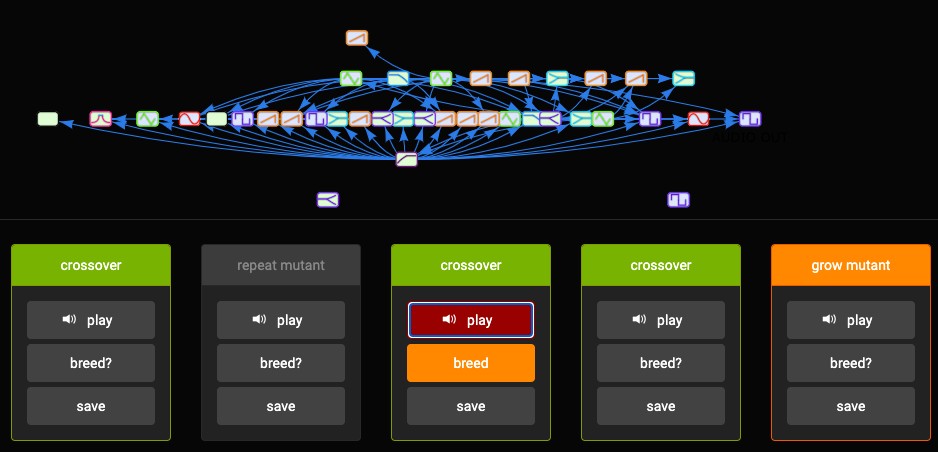
\includegraphics[width=0.95\textwidth]{figures/background/EvoSynth.png}
    \caption{EvoSynth. A web-based interface for an interactive evolutionary approach to programming a software modular synthesizer. Users are presented with a selection of potential sytnhesizer patches generated using concepts inspired by evolutionary biology. They can listen to these patches and refine them through "breeding" which creates mixtures of multiple patches.}
    \label{fig:evosynth}
\end{figure}

Scurto \textit{et al.} \cite{scurto2021designing} explored interactive machine learning for parameter selection using a deep reinforcement learning (RL) algorithm \cite{sutton2018reinforcement}. They developed \textit{Co-Explorer}, an RL algorithm that was able to accept feedback from the user and generate new synthesizer parameter settings in response. Co-Explorer supported both binary feedback, e.g., "I like / don't like that result", as well as \textit{zone feedback} which could be used to direct the algorithm into or away from a particular zone of the parameter space. Users were also able to guide the system using \textit{state commands} such as tell the system to move to a previous setting, enter into an autonomous exploration mode, or allow users to take over control completely.

One of the benefits of evaluation-based systems is that they re-engage users in the process of searching for parameter settings, as opposed to taking over control of entire process as in the case in example-based interaction paradigms. These types of interfaces may be beneficial, especially when the user does not have an example sound for the system or wants to use a more exploratory approach.

\section{Using Descriptive Words}\label{section:descriptive-words}
In 1986 Ashley proposed one of the first examples of an system for programming a synthesizer using semantic descriptions of the desired timbre \cite{ashley1986knowledge}. Shortly after Ethington published the SeaWave system which enable timbral control using predefined adjectives \cite{ethington1994seawave}. SeaWave broke the timbre of a sound into three different overlapping temporal segments (attack, presence, and cutoff) and mapped various adjectives within each of these segments to parameters of an additive synthesis engine. Johnson \textit{et al.} proposed a machine learning approach to mapping timbral descriptors to parameter settings \cite{johnson2006timbre}. Ross Clement collected a set of human-made Yamaha DX7 presets and extracted keywords from the names of the presets to help develop a preset generation system based on the most commonly found keywords \cite{clement2011automatic}. A novel approach to using descriptive words proposed by Krekovi\'{c} \textit{et al.} \cite{krekovic2016algorithm} first used a combination of an expert-based system that mapped adjectives to numerical values for target audio features, and then used a GA to search for a parameter that matched those audio features. Figure \ref{fig:krekovic-desc} shows a diagram of this system.

\begin{figure}[ht]
    \centering
    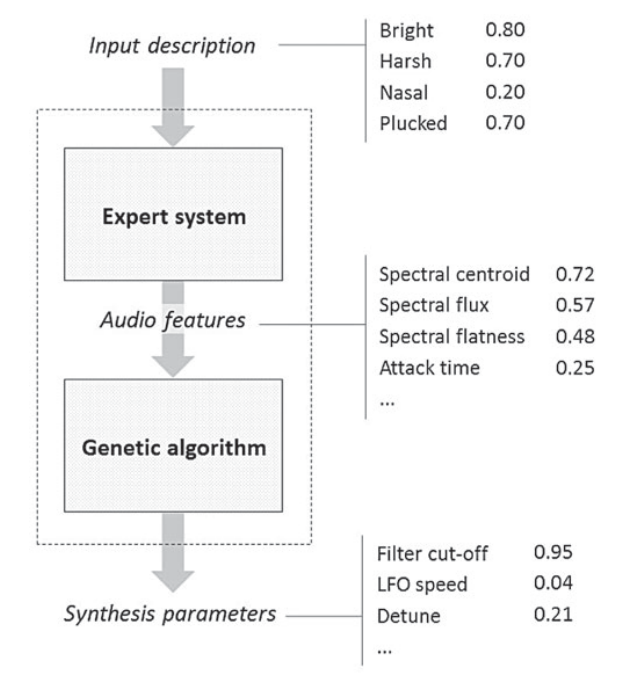
\includegraphics[width=0.5\textwidth]{figures/background/krekovic-descriptive.png}
    \caption{Krekovi\'{c} \textit{et al.}'s \cite{krekovic2016algorithm} system for mapping between timbral descriptions and synthesizer parameter settings. }
    \label{fig:krekovic-desc}
\end{figure}

% - Ben Hayes work fits in here. 
% % Does this is fit in on the topic of synthesizer timbre?? Or perhaps there is an opportunity to discuss the timbre space in representations? Representing synthesizer sounds or something?
% % - Research by Benjamin Hayes on the timbre space of synths -- looks super interesting.
% % - https://benhayes.net/assets/pdf/16.Hayes.pdf
% % - https://benhayes.net/assets/pdf/icmpc_escom_2021.pdf
% % - https://benhayes.net/publications/ (Has some interesting perceptual studies on synthesizer timbre space, also something new on neural synthesis)

% Definitely need to review and cite this \cite{wallmark2019creating}

In a recent study, Roche \textit{et al.} explored controlling synthesis using eight perceptually motivated parameters \cite{roche2021make}. Their work used a neural synthesizer that generated spectrograms using a variational autoencoder (VAE) regularized using perceptual attributes to provide parameters based on timbral descriptions. Although this work does not fit the traditional description of automatic synthesizer programming since the mapping is not made to the parameter space of a regular DSP synthesizer, their method provides a good framework for exploring perceptually motivated controls for audio synthesis and could likely be applied to other, more traditional forms of synthesis.

In related work, Hayes and Saiti explored the semantic dimensions of a three operator FM synthesizer \cite{hayes2020there}. %In their study, experienced sound designers were asked to program a synthesizer, starting from a preset, in order to create a sound that fulfilled a timbre objective related to the luminance-texture-mass (LTM) model of timbre semantics (e.g. brighter, less thick, more rough, ..., etc.). Users were then asked to rate sounds based on a larger selection of timbre adjectives. 
They found five major factors related to timbre semantics; the first two factors related to the  luminance-texture-mass (LTM) model of timbre semantics \cite{zacharakis2012interlanguage} and the additional three factors related to clarity, pluckiness, and rawness.


\section{Vocal Imitations}
A method that has been shown as an effective way to communicate sound concepts is by using vocal imitations \cite{lemaitre2014effectiveness}, and is more effective than using a verbalization in the case of unidentified sounds (sounds that have an unclear source). Building on this, Cartwright \textit{et al.} developed the VocalSketch dataset \cite{cartwright2015vocalsketch} to support research in using vocal imitations to communicate sound concepts to computers. In synthesizer programming, the vocal imitation approach can be viewed as a subset of the example-based interface approaches as vocal imitations are a specific style of examples that could be provided to a system.

Cartwright \textit{et al.} proposed the SynthAssist system for exploring and finding synthesizer sounds through vocal imitations \cite{cartwright2014synthassist}. Using SynthAssist a user can record an imitation of the synthesizer sound they wish to play and be presented with a set of possible solutions. They can then enter into an evaluation-based interaction style where the can rate and iterate through alternative sounds until they find a match. SynthAssist uses a data-driven approach for retrieving candidate synthesizer patches. A large number of patches are pre-generated and a set of time-series audio features are computed and stored in a database along with the parameter settings and audio. Candidate synthesizer settings are queried using dynamic time warping to compare the audio feature time-series. 

% TODO
%[maybe add an example of the SynthAssist interface]

% What's this cite? \cite{blancas2014sound}

In related work, Zhang \textit{et al.} recently released \textit{Vroom!}, a sound search engine based on vocal imitations \cite{zhang2020vroom}. \textit{Vroom!} builds off of previous work by Zhang on query sounds by vocal imitations using CNNs \cite{zhang2017iminet, zhang2018visualization}. The implemented network features a siamese CNN stack that extracts audio features from the vocal imitation and sound target in parallel and then uses a fully connected layer to compute similarity.

\section{Intuitive Controls}
%Possible candidates for additional work \cite{dahlstedt2001creating}, \cite{arfib2002strategies}, \cite{huang2014active}
The idea of developing more intuitive controls that overlay the more complex low-level parameter space was introduced by Wessel in 1979 \cite{wessel1979timbre}. Wessel proposed a system based on Grey's timbre space \cite{grey1977multidimensional} for controlling an additive synthesizer using two higher-level perecptual parameters arranged on a two-dimensional grid: the vertical axis was related to the spectral energy distribution and the horizontal axis was related to the character of the attack. Adjusting these parameters lead to smooth perceptual transitions. Wessel suggested a method for achieving more complex forms of control, based on an efficient computer language.

The descriptive words-based application proposed by Krekovi\'{c} that was previously mentioned \cite{krekovic2016algorithm} also serves as an example of a system that uses intuitive controls. The input to that system is a set of numerical values associated to timbral descriptors, which are then used to program a synthesizer. This input can be thought of as a set of high-level intuitive parameters that operate at the semantic space of the user; the system is responsible for connecting these timbral parameters to the underlying synthesizer parameters.

\subsection{Learning Controls}
% Read these papers plus nsynth to get a bit more context for the macro parameters
% Does this fit in here: \cite{tatar2021latent} ?
% Want to cite some of the neural synthesis approaches too
Recent work with generative models in the deep learning space has also proposed systems that expose intuitive \textit{macro} parameters to a user \cite{esling2020flow, roche2021make, le2021improving}. The auto encoder style networks that have been used for these approaches features a latent space in the architecture that provides a learned compact representation of the input. New examples can be generated by sampling this latent, which is why these approaches are called generative approaches. Each variable within the latent space can be thought of as a new higher-level macro parameter for a synthesizer that contains a complex and non-linear mapping to one or more of the underlying synthesizer parameters. One of the issues with these approaches is that the relationship between the latent parameters and synthesizer parameters is challenging to understand, and what each of the latent parameters does is not completely clear. Roche has taken steps towards creating a perceptually relevant latent space by regularizing the parameters to have correlates with timbral descriptors \cite{roche2021make}.

\section{Exploration Interfaces}
Exploration interfaces support finding potential solutions or alternatives. These types of interfaces have been introduced in related fields including intelligent music production to facilitate finding audio mixing parameters \cite{cartwright2014mixploration} or to help browse for audio samples \cite{fried2014audioquilt, shier2021manifold, turquois2016exploring}. Many of the previously mentioned automatic synthesizer programming tools can also be categorized as exploration interfaces. Interactive genetic algorithms help facilitate exploration by iteratively allowing users to listen to and evaluate sets of sounds from a synthesizers space of sounds \cite{johnson1999exploring, dahlstedt2001creating, yee2016use}. The genetic algorithm approach to inverse synthesis proposed by Masudo \textit{et al.} supported exploration by emphasizing diversity as well as close matches in the set of possible solutions presented to users \cite{masudo2021quality}. This meant that users would be presented with a set of diverse potential options when searching for a synthesizer setting. The reinforcement learning approach proposed by Scurto \textit{et al.} helps to facilitate a structured approach to parameter exploration \cite{scurto2021designing}. 

Interfaces that visualize sounds on two or three dimensional interfaces based on sound similarity, such as the timbre space representation proposed by Wessel \cite{wessel1979timbre}, provide an embodied approach to exploring synthesizer sounds by activating visual and spatial cognition in addition to auditory cognition. The benefit of embodied cognition to creative practices is identified by Davis \textit{et al.} \cite{davis2013toward} and visualization of synthesizer sounds based on sound similarity is explored in more detail in chapter \ref{chapter:synth-explore}. SynthAssist also uses a visual layout of synthesizer sounds to support users in exploration \cite{cartwright2014synthassist}.

Another type of interface that enables exploration are graphical interfaces, which allow users to interpolate between synthesizer presets \cite{gibson2020analyzing}. These systems generally present a user with a two-dimensional interface that represents a number of different presets for an underlying synthesis engine. Each preset is positioned in a different location on the interface and the user can specify a point on the interface resulting in an interpolation between presets represented at that position. Le Vaillant \textit{et al.} conducted a user evaluation that compared a users ability to recreate a sound using an interface with four parameters that controlled a synthesis engine against a graphical interpolation interface \cite{le2020analytic}. Expert users were able to use both interfaces equally well; however, novice and intermediate users were able to match the sound more easily and achieve comparable results to expert users with the interpolating interface.

% Not positive if I should include this
% \section{Bridging the Conceptual Gap}
% % Maybe move this up into the exploratory interfaces? This can be like "related work on finding timbre space specifically for synthesized sounds of something like that"
% All the work mentioned in previous sections seeks to bridge the conceptual gap between the perceptual / semantic space and the parameter space of a synthesizer. The body of work that has been conducted to this end further reinforces the complexity of the divide. Developing a deeper understanding of the relationship between these spaces will enable future work in automatic synthesizer programming. Research specifically focused on developing a deeper understanding of this area has been conducted. Vahidi \textit{et al.} found correlations between the timbre space of subtractive synthesizer and a set of low-level audio features \cite{vahidi2020timbre}. Similar to Grey \cite{grey1977multidimensional}, they used multi-dimensional scaling (MDS) to produce a timbre space representation for a set of synthesized tones and found high perceptual correlations with certain spectral features. 

%  \subsubsection{Others}
%  Sketching sounds \cite{lobbers2021sketching} \cite{knees2016searching}
 

\section{Conclusions}
This chapter has introduced the topic of automatic synthesizer programming and presented a review of related work. This review framed the \textit{synthesizer programming problem} as a human-computer interaction problem and organized the body of automatic synthesizer programming research from this perspective. Six difference user interaction methods were identified and include: 1) example-based interfaces, 2) evaluation interfaces, 3) using descriptive words, 4) vocal imitations, 5) intuitive controls, and 6) exploration interfaces. All of these approaches have a common goal of assisting synthesizer users in navigating the disconnect between synthesizer parameters and the resulting auditory result.

Example-based interfaces allow users to specify a desired auditory output from their synthesizer by providing an example sound to an automatic synthesizer programming interface. These methods utilize inverse synthesis or sound matching to predict synthesizer parameters to match a target sound, and represent a large portion of the automatic synthesizer programming literature. Evolutionary programming has dominated the landscape of related work until recent years, which has seen a rise in deep learning approaches. User studies have identified example-based systems as being considered useful by synthesizer users \cite{krekovic2019insights} and as such are a focus of the next two chapters in this thesis. Chapter \ref{chapter:spiegelib} describes an open-source library that was developed as a part of this thesis to support further research and shared evaluations. Chapter \ref{chapter:inverse_synth_experiment} presents an evaluation of several deep learning and genetic algorithm based methods for a baseline FM synthesizer inverse synthesis problem.

The emphasis placed on example-based interactions and inverse synthesis do not necessarily indicate that these approaches are the best solutions to the synthesizer programming problem. Evaluation and exploration-based interfaces and intuitive controls are beneficial as they engage the user in the process of selecting synthesizer sounds as opposed to completely taking over control, as is the case with example-based interfaces. The use of descriptive words and vocal imitations also represent ways that musicians already communicate music ideas to each other and could provide promising approaches for designing intuitive user interfaces \cite{pardo2019learning}. 

The best interface will likely vary depending on the specific user and their specific needs for a given creative project. Some users may have a specific idea of what they want while others may be searching for inspiration \cite{andersen2016conversations}. As a result, developing interfaces that support a variety of different interaction styles will likely be beneficial. Building on these concepts, a prototype for an exploration-based automatic synthesizer programming interface is described in chapter \ref{chapter:synth-explore}, which was designed based on a set of proposed design criteria derived from the fields of creativity support tools \cite{shneiderman2007creativity} and music interaction \cite{holland2013music}.

% From this disconnect arises a conceptual gap between the space of synthesizer parameters and the perceptual / semantic space of the user. 


% - Okay can I motivate future work here?
% - The parameter space is ginormous! How do we represent synthesized sounds in a perceptually relevant way? The relationship between parameters and the resulting output sounds is very complex. Deep learning 

% Challenges. Maybe move this to a section that is specifically related to automatic synthesizer programming challenges.
% This is a challenge that is potentially particularly related to synthesizer programming. The space of possible sounds is immense! It is infeasible to compute all the possible sounds and index them beforehand. So the question becomes, how to you navigate this space in an intelligent way?? How do we learn to teach our systems to generate sounds or learn to programm sounds in a way that is related to or relevant to how a human would program a sound?? This is addressed in the torchsynth chapter a bit.
% One of distinguishing factors between querying tasks and automatic synthesizer programming is that often querying tasks, the database of audio already exists and can be queried for an exact match or for the match that is most similar. Some approaches to automatic synthesizer programming have pre-computed large sets of sytnhesizer sounds 




% A related field in HCI is Music Interaction \cite{holland2013music}.

% \subsection{Synthesizer Users}
% Davis \textit{et al.} focus on the role that CSTs play in supporting novices engaging in creative tasks and the relationship that the environment plays in creativity \cite{davis2013toward}. In their work, the authors identify two types of novice users: domain novices and tool novices. Domain novices are new to both the creative domain as well as using the creativity support tool. Tool novices have experience with the creative domain, but are novices at using a particular tool. Both types of novices described by Davis \textit{et al.} are common and serve to benefit from the development of improved methods for interacting with them; domain novices are both new to sound design / music production as well as to using a specific synthesizer, whereas a tool novices would likely have experience with sound design / music production, but would be a novice with using a specific synthesizer.







% % Should this go into the previous chapter?
% Automatic synthesizer programming is fundamentally attempting to solve a human computer interaction (HCI) problem: "How can a synthesizer user more effectively communicate their creative ideas to a synthesizer?" Pardo \textit{et al.} described the challenges with using music production tools (a synthesizer is a type of music production tool) as resulting from the large conceptual gap between the parameters and perceptually relevant output from the tool \cite{pardo2019learning}. To be more precise, Pardo \textit{et al.} describe the specific conceptual spaces that are involved in interacting with a music production tool: the perceptual space, the parameter space, and the semantic space. The perceptual space is related to how a tool actually sounds when it is being applied, i.e. we can tell the different when the filter on synthesizer is changed. The parameter space is the actual low-level techniques parameters on the control interface, i.e. the filter was parameter changed from 500Hz to 2000Hz. The semantic space is related to how one would describe the changes that we hear, e.g the synthesizer sounds brighter as a result of the filter change. Complexities with using a synthesizer arise when users are asked to bridge the gap between the low-level parameter space and the higher-level perceptual and semantic spaces themselves, which often involves a complex and non-linear mapping. Pardo \textit{et al.} identify the novice user as being particularly challenged by gap between the low-level and high-level spaces, and present a framework for developing tools that help to bridge that gap. 

% Despite the large body of work that has been conducted in automatic synthesizer programming, there exists no literature that overviews and organizes the related work. In this chapter I provide an overview of the field of automatic synthesizer programming and use the framework presented by Pardo \textit{et al.} to organize previous work using a human computer interaction lens. Due to the large body of related work in inverse synthesis, and its importance to experiments conducted in this thesis, particular emphasis is paid to the various algorithmic approaches that have been explored. The remainder of this chapter is structured as follows: [fill this in]

%--------------------------------------------------------------------

% \section{Background}
% \label{sec:asp-background}
% Automatic synthesizer programming is an inherently interdisciplinary field. Previous research has focused on both the algorithmic and technical aspects of the problem, as well as the human interaction aspects of the problem. Depending on the focus a solution may draw from fields including human-computer interaction, digital signal processing (DSP), machine learning and artificial intelligence, to name a few. Insights can also be gleaned from related fields including music information retrieval and intelligent music production. To provide context and situate automatic synthesizer programming in a wider body of research, a brief introduction to these fields and how they relate to the synthesizer programming problem is provided in this section.

% \subsection{Human Computer Interaction}
% \subsubsection{Creative Support Tools}
% Automatic synthesizer programming can be viewed from the perspective of trying to solve a human computer interaction (HCI) problem. How can a synthesizer user more effectively communicate their creative ideas to a synthesizer? Currently users are expected to learn the domain language from the perspective of whatever synthesis algorithm they are using. Can a user instead communicate their ideas to a synthesizer in a way that fits their creative needs? Creativity support is an emerging field of study that is interested in answering questions similar to this. It is focused on the development of tools that enable and enhance the creative output of an individual or group, both novices and experts. Creativity support tools (CSTs) \cite{shneiderman2007creativity} span a wide array of application domains including visual art, textiles, cooking, and music. A central question that CSTs ask is: 
% \begin{quote}
%     "How can designers of programming interfaces, interactive tools, and rich social environments enable more people to be more creative more often?"
% \end{quote}

% Too much detail - maybe put this in the last chapter
% Shneiderman \cite{shneiderman2007creativity} outlines a set of design principles for developing creativity support tools which include: support exploratory search, enable collaboration, provide rich history keeping, design with low thresholds, high ceilings, and wide walls. In subsequent related work, Davis \textit{et al.} focus on the role that CSTs play in supporting novices engaging in creative tasks and the relationship that the environment plays in creativity \cite{davis2013toward}. In their work, the authors identify two types of novice users: domain novices and tool novices. Domain novices are new to both the creative domain as well as using the creativity support tool. Tool novices have experience with the creative domain, but are novices at using a particular tool. To help evaluate and promote the development of creativity support tools for novices, they also propose a theory of creativity support based on cognitive theory.

% These concepts provide an important platform for beginning to develop tools to support users of synthesizers. Both types of novices described by Davis \textit{et al.} are common and serve to benefit from the development of improved methods for interacting with them; domain novices are both new to sound design / music production as well as to using a specific synthesizer, whereas a tool novices would likely have experience with sound design / music production, but would be a novice with using a specific synthesizer.

% This is also a bit too in detail
% \subsubsection{Music Interaction}
% Music and Human-Computer Interaction \cite{holland2013music}, or Music Interaction. Research related to the use of interactive systems that involve computes for any kind of musical activity. Music interaction draws heavily from other areas of HCI research, but also responds to the needs and desires of the music community. There are unique considerations in the context of musical applications that makes music interaction different from other fields of HCI. A musical instrument is not a utilitarian tool whose development should be ever-improved to make it more efficient. Musical instruments are played, and sometimes that is the only goal. Tomaka [cite me!] identifies that imperfections and limitations of a musical instrument give an instrument character. McDermott \cite{mcdermott2013should} identifies the importance of engagement in musical interaction and the relation that bears to the concept of \textit{flow} \cite{csikszentmihalyi1990flow}. The learning curve plays is crucial to the level of engagement that a player experiences when playing a musical instrument, both in the short-term and long-term. Holland \cite{holland2013music} concludes, "In order to remain engaging, consuming and flow-like, activities that involve musical instruments must offer continued challenges at appropriate levels of difficulty: not too difficult, and not too easy."

% \subsubsection{Music Production Tools}
% Related to musical instruments are tools that are used in the process of recording and producing musical recordings. Music producers often use a collection of computer-based music production tools including DAWs, audio plugins, and synthesizers to create their musical compositions. In fact, the term \textit{in-box} has been coined to refer to the process of creating a piece of music from start to finish completely within a computer. With the rise of more music production tools and libraries of sounds for creating music with (often referred to as audio sample libraries), producers have started to express desire for improved methods of interaction. Kristina Andersen conducted a set of interviews with expert music producers at the Red Bull Music Academies in 2014 and 2015, and asked them about their experience with their music production tools \cite{andersen2016conversations}. One of the main challenges expressed was related to navigating large collections of audio libraries, which could contain half a million or more individual audio files. A main finding that reflects some of the principles of music interaction is that some participants relied on idiosyncratic methods as well as randomness; serendipity played a role in their creative process and they expressed a desire for tools that would support that. Another interesting finding is that users often had a mental image of their creative vision, creating tools that could interpret those, whether through semantic descriptions, colours, images, or haptics would be a valuable interaction paradigm. 

% Pardo \textit{et al.} \cite{pardo2019learning} breakdown the current interaction paradigm for music production tools into three different conceptual spaces: the perceptual space, the parameter space, and the semantic space. The perceptual space is related to how a tool actually sounds when it is being applied, i.e. we can tell the different when the filter on synthesizer is changed. The parameter space is the actual low-level techniques parameters on the control interface, i.e. the filter was parameter changed from 500Hz to 2000Hz. The semantic space is related to how one would describe the changes that we hear, e.g the synthesizer sounds brighter as a result of the filter change. Users are asked to bridge the gap between the low-level parameter space and the higher-level perceptual and semantic spaces themselves, which often involves a complex and non-linear mapping. Pardo \textit{et al.} identify the novice user as being particularly challenged by gap between the low-level and high-level spaces, and present a framework for developing tools that help to bridge that gap. They propose four different methods for doing so: 1) Evaluation (allow the user to listen and evaluate a set of proposed variations), 2) using descriptive words, 3) using vocal imitations, and 4), exploration.

% % This creates some design motivation / questions specific for ASP.
% \subsubsection{HCI and Automatic Synthesizer Programming}
% The inverse synthesis approach seeks to completely abstract the process of programming a sound. Creating a new sound with a synthesizer is seen as a hindrance to the process of creating music. But people enjoy using synthesizers and being involved in the process of designing new sounds. They already support long-term engagement to the dedicated users. The question arises, how can we support creativity and engagement for users of all experience levels? Can interfaces be designed that offer continued challenges at the appropriate level of difficulty? Can these interfaces adapt to the correct level of difficultly for a particular user?

% With the mass digitization of musical recordings and the shift to producing music with computers, questions around how we interact with music via computers have grown. Several related fields of study, adjacent to automatic synthesizer programming, have emerged over the years in attempt to answer these questions. Contributions from these fields provide insight into the larger trends in music interaction as well as provide inspiration for future directions in synthesizer programming. Two particularly related fields worth mentioning is music information retrieval (MIR) and intelligent music production.

% \subsection{Music Information Retrieval}
% MIR is a growing research area that was born out of the need to navigate increasingly large collections of digital music. The field centers around the International Society of Music Information Retrieval (ISMIR), created through the merging of the fields of symbolic music and audio signal processing in 1999, hosted their first annual symposium in 2000 \cite{downie2009ten}. One of the main research goals of MIR is to develop systems to support users in organizing and querying large collections of digital audio. A number of unique solutions to querying audio databases have been proposed including query-by-example \cite{zloof1977query}, query-by-vocal-imitation \cite{blancas2014sound}, and query-by-beat-boxing \cite{kapur2004query}. Automatic synthesizer programming can be viewed as a query retrieval task where the product being retrieved is a parameter setting for a particular synthesizer. Query-by-example is directly related to the inverse synthesis problem and others have proposed query-by-vocal-imitation for automatic synthesizer programming as well \cite{cartwright2014synthassist}. 

% Visualization of audio databases to support navigation and browsing is another established area of research in MIR. One of the first researchers to explore visualizations of audio based on timbre was Grey \cite{grey1977multidimensional} in 1977, followed by subsequent work by Wessel in 1979 \cite{wessel1979timbre}. The concept of visualization in MIR is comprehensively reviewed by Cooper et al. \cite{cooper2006visualization}, and is updated by Schedl et al. to represent contemporary work \cite{schedl2014music}. AudioQuilt is a notable example of an experimental application for visualizing audio samples \cite{fried2014audioquilt}. AudioQuilt uses metric learning and kernalized sorting algorithms to visualize audio samples in two dimensions. Tzanetakis and Cook \cite{tzanetakis20003d} review experimental applicationts with novel user interfaces for exploring sound collections in three dimensions. A unique approach to sample retrieval is proposed by Knees and Andersen \cite{knees2016searching}, in which users query audio using visual sketches of their mental images of that sound.  Visualization of synthesizer sounds is explored in chapter 

% \subsection{Creative MIR and Intelligent Music Production}
% Creative MIR is a subset of MIR that is focused on the applying techniques from the field towards creative applications including music production \cite{humphrey2013brief}. Music production tools, including tools to that support querying and browsing of a audio samples and synthesizing new sounds are an aspect of this. Expert music producers have expressed desires for improved methods for working with large collections of audio samples \cite{andersen2016conversations} as well as for the development of systems that would help generate novel ideas. 

% Music producers have expressed desires for improved methods for working with  Related work that I completed during my time at University of Victoria focused on techniques for visualizing drum machine samples in a music production context \cite{shier2021manifold}. Intelligent music production \cite{moffat2019approaches} is another related field that draws from MIR and machine learning with the aim to develop tools that support creativity and automate workflows within the context of music production. Tools that automate mixing, the practice of combining multiple individual audio tracks into a single tack, is a complex task that has received a large amount of focus \cite{de2017ten}.


% \subsection{Neural Synthesis}
% One area of new development in audio synthesis is in methods that are leveraging advancements from the field of deep learning [deep learning cite], an area of audio synthesis that is explored in this thesis.  
% In contrast to traditional synthesis, neural synthesizers generate audio using large-scale machine learning architectures with millions of parameters \cite{engel2017neural}. Differentiable digital signal processing \cite{engel2020ddsp} bridged the gap between traditional DSP synthesizers with the expressiveness of neural networks, exploring a harmonic model-based approach, using a more compact architecture with 100K parameters.
% One benefit of synthesized audio is that the underlying factors of variation ({\em i.e.}~the parameters) are known.

% % GANs for synthesis
% In this work, we use Generative Adversarial Networks (GANs) \cite{goodfellow2014generative} to generate new instrumental audio from a dataset of existing material. GANs have the potential to be used to generate new sounds on the fly. This would dramatically alleviate both the problem of having to pore through giant sound libraries, and the problem with having to only use one sample repeatedly. In addition, the explosion of new sounds which could potentially be produced by GANs would vastly reduce recording costs by designers of sound libraries.

% This research avenue is to a certain degree untapped: GANs have been successfully applied to the generation and manipulation of images, however, relatively little work has been focused on the audio domain. Research related to the specific work proposed here was presented by \cite{donahue2018adversarial}  and \cite{engel2018gansynth}.
% \cite{ccakir2018musical} - not totally sure what this is about, I think it is generative though.

%--------------------------------------------------------------------

- 